\section{BSM Physics at a High Luminosity LHC with ATLAS}

\begin{frame}
\frametitle{BSM Physics at a High Luminosity LHC with ATLAS}
\begin{itemize}
    \item It is also important to plan for future upgrades to both the
        ATLAS detector and the LHC itself.
    \item Understanding the expected sensitivity to BSM processes under
        various upgrade scenarios is necessary for to
    \begin{itemize}
            \item prioritize detector and collider development
                projects
            \item plan the scope of the next generation of collider
                experiments.
    \end{itemize}

    \item Upgrade scenarios to the ATLAS detector and the LHC are
        considered, with up to 3000~fb$^{-1}$ delivered---10x Run II
        predictions.

\item The feasibility studies presented were included in
    \begin{itemize}
    \item the ATLAS submission to the European Strategy Meeting
    \item ATLAS Phase-II Letter of Intent
    \item the Snowmass effort
    \end{itemize}
\end{itemize}
\end{frame}

\subsection{Software}

\begin{frame}
    \frametitle{Software}
    \begin{itemize}
\item I developed the software framework for the feasibility studies.
\item Designed in modules to accommodate the range of analyses carried
    out while keeping as much as possible common across analyses

\item Four stages of analysis corresponding to software modules:
    \begin{itemize}
        \item event generation and parton showering (\pythia)
        \item object selection
        \item event selection
        \item plotting and limit setting
    \end{itemize}

\item A mixture of C++ and python was used.
\item Interfaces to \pythia\ (for parton showering), FastJet (for jet
    clustering), and BAT (for limit setting) were implemented.
\end{itemize}

\end{frame}

\subsection{Exotic Dilepton and \ttbar\ Resonances}

\begin{frame}
    \frametitle{Exotic Dilepton Resonances}
\centering
\begin{figure}
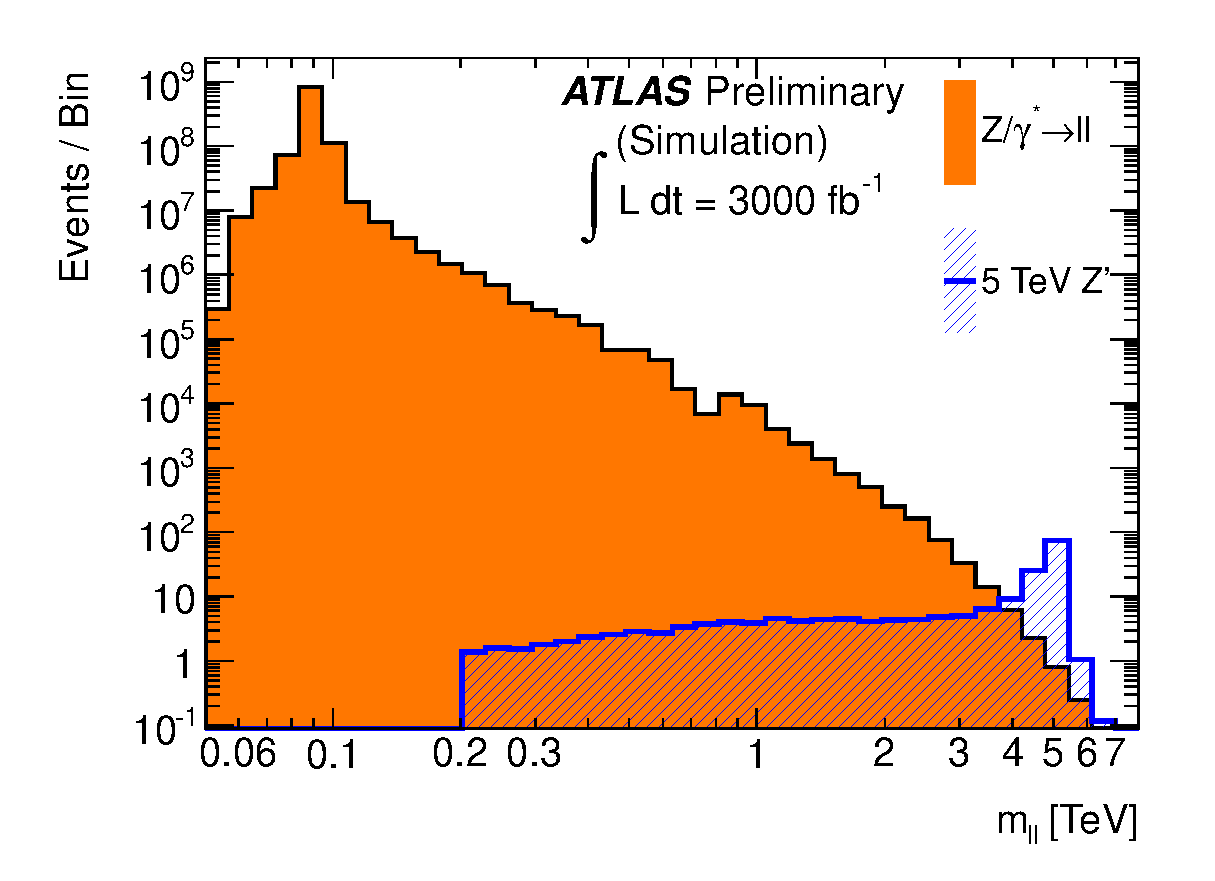
\includegraphics[width=.5\textwidth]{signal_background_log10_m_ll_zprimeelel5000_log.eps}
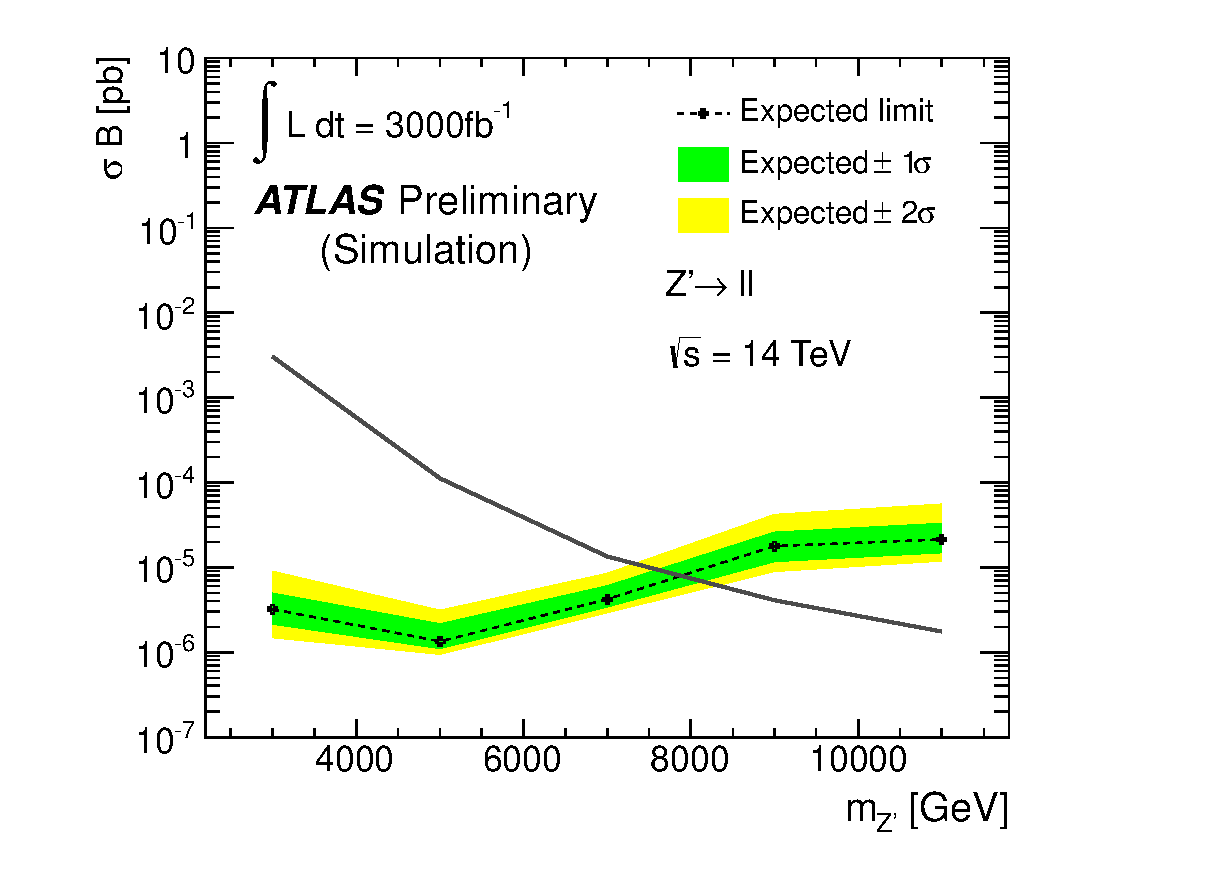
\includegraphics[width=.5\textwidth]{zprimeelelxsec_Log_3000fb.eps}
\end{figure}

\begin{tabular}{lccc}
\hline
model              & $300\,\ifb$  & $1000\,\ifb$     & $3000\,\ifb$  \\
\hline
\hline
$Z^\prime_{SSM} \to ee$ & 6.5  & 7.2   & 7.8   \\
$Z^\prime_{SSM} \to \mu \mu$ & 6.4  & 7.1   & 7.6   \\
\hline
\end{tabular}
\vspace{5pt} \\
\noindent Expected limits (TeV) for various upgrade scenarios
\end{frame}

\begin{frame}
    \frametitle{Exotic \ttbar\ Resonances}
\centering
\begin{figure}
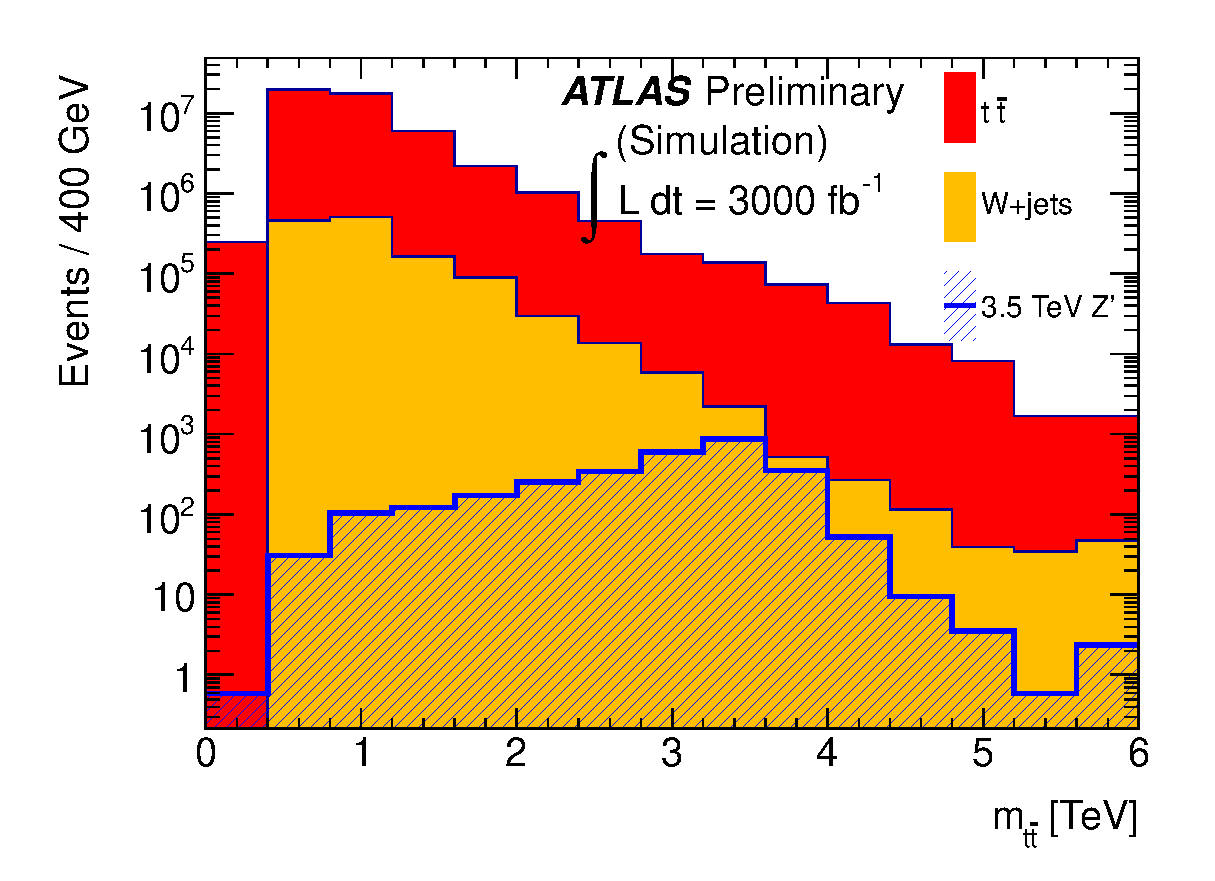
\includegraphics[width=.5\textwidth]{signal_background_ljets_mass_zprime3500_log.eps}
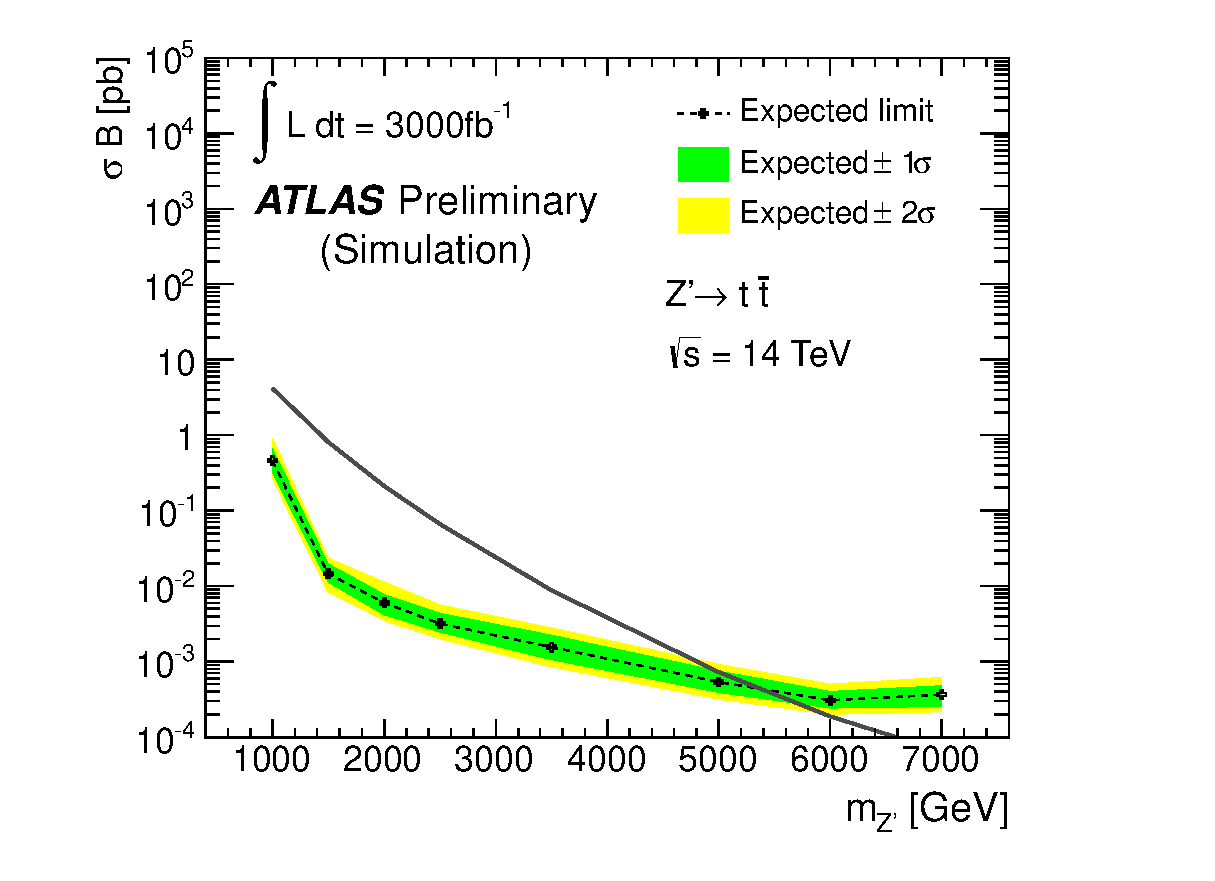
\includegraphics[width=.5\textwidth]{zprimexsec_Log_3000fb.eps}
\end{figure}

\begin{tabular}{lccc}
\hline
model              & $300\,\ifb$  & $1000\,\ifb$     & $3000\,\ifb$  \\
\hline
\hline
$g_{KK}$ & 4.3 & 5.6 & 6.7 \\
$Z^\prime_{\rm topcolor}$ & 3.3 & 4.5 & 5.5 \\
\hline
\end{tabular}
\vspace{5pt} \\
\noindent Expected limits (TeV) for various upgrade scenarios
\end{frame}
